The global model was used to infer the electric field, electron densities, and
electron temperatures in the \acs{rpnd} from the metastable measurements.
However, as was described in the development of the model, it is also capable of
predicting the densities of other excited states and the optical emissions of
the \acs{rpnd}. This chapter will describe the measurement of the optical
emissions of the \acs{rpnd} and then the use of these measurements to determine
the \acs{rpnd} wave velocity and electrons temperatures. Finally, the electron
temperatures and the spectral trends will be compared to those obtained from the
global model.

\section{Emission Measurements}

Emissions spectroscopy was conducted at the same operating conditions as the
metastable measurements. Light collection was accomplished with a 1 cm diameter
bundle of optical fibers, butted against the outside of the glass envelope. The
other end was placed at the entrance slit of a ISA Jobin-Yvon SPEX HR460
monochromator. A grating with 1200 grooves/mm was installed in the
monochromator. The entrance slit width was set to 250 $\mu$m and the exit slit
was set at 500 $\mu$m. This was done so as to collect the integrated intensity
of each spectral line.

A photomultiplier tube (\acs{pmt}) of model C31034 was used to record the
changes in intensity over time. The tube voltage was set to 1900 V and was
terminated into a 50 $\Omega$ resistor. Specifications could not be found for
the tube, however measurements demonstrated a rise time of, at most, 3.5 ns.

The range of spectral sensitivity for the photocathode of the \acs{pmt} limited
measurements to transitions occurring between 350-750 nm. The list of observable
transitions is recorded in table~\ref{tbl:transitions}.
\begin{table}
  \centering
  \caption{Table of the observed optical transitions and their transition
    rates.}
  \begin{tabular}{lllll}
    \toprule                                                                    \\
    Initial      & Final        & Wavelength &              &                   \\
    State        & State        & (nm)       & A (s$^{-1}$) & $\sum$A (s$^{-1}$)\\
    \midrule                                                                    \\
    3$^3$P$\odd$ & 2$^3$S       & 388.97     & $9.46\EE6$   & $1.06\EE7$        \\
    4$^1$P$\odd$ & 2$^1$S       & 396.59     & $6.95\EE6$   & $2.52\EE8$        \\
    5$^3$D       & 2$^3$P$\odd$ & 402.73     & $1.16\EE7$   & $1.64\EE7$        \\
    4$^3$D       & 2$^3$P$\odd$ & 447.28     & $2.46\EE7$   & $3.12\EE7$        \\
   %4$^3$S       & 2$^3$P$\odd$ & 471.45     & $9.52\EE6$   & $1.60\EE7$        \\
    4$^1$D       & 2$^1$P$\odd$ & 492.33     & $1.99\EE7$   & $2.70\EE7$        \\
    3$^1$P$\odd$ & 2$^1$S       & 501.71     & $1.34\EE7$   & $5.80\EE8$        \\
    3$^3$D       & 2$^3$P$\odd$ & 587.73     & $7.07\EE7$   & $7.07\EE7$        \\
    3$^1$D       & 2$^1$P$\odd$ & 668.00     & $6.37\EE7$   & $6.37\EE7$        \\
    3$^3$S       & 2$^3$P$\odd$ & 706.72     & $2.79\EE7$   & $2.79\EE7$        \\
    3$^1$S       & 2$^1$P$\odd$ & 728.34     & $1.83\EE7$   & $1.83\EE7$        \\
  \end{tabular}
  \label{tbl:transitions}
\end{table}



\section{Wave Velocities}

In the analysis of \acs{fiw} discharges, one of the most common means of
comparison is the use of wave velocities. In the studies reported by Vasilyak
\cite{Vasilyak1994}, the velocities were measured using several approaches. In
one, capacitive probes were placed in contact with the dielectric of the
discharge tube, and the time delay between the voltage signals was used as the
wave velocity. In some cases an intensified \acs{ccd} was used to track the
propagation of the wave. Alternately, a photomultiplier tube was positioned
against the dielectric at varying axial locations. This is the approach used
here.

The maximum detectable velocity was limited by several factors. Data were only
available at intervals of 1 ns. As the maximum separation of measurement
locations was 15.24 cm, this set an upper limit of about 1.5$\times10^8$ m/s.
Additional limitations were imposed by the jitter of the pulser output. Overall,
the maximum detectable wave velocity was $5.0\times10^7$ m/s.

The velocities were determined as an average of the all the emission curves
recorded. In each case, the curve at each axial location was interpolated with a
smoothing spline. The time of the maximum derivate of the emission curves was
used as the reference point in each case. The distance between the measurement
locations was then divided by the time delay between the maximum derivatives.
The results of these calculations are recorded in table~\ref{tbl:velocities}.
\begin{table}
  \centering
  \caption{Wave velocities in the \acs{rpnd}.}
  \label{tbl:velocities}
  \begin{tabular}{lll}
    \toprule                                                      \\
    Pressure  & Upstream                & Downstream              \\
    (Torr)    & Velocity (m/s)          & Velocity (m/s)          \\
    \midrule                                                      \\
    8.0       & $3.01\pm1.21\times10^7$ & $1.73\pm0.26\times10^7$ \\
    16.0      & $1.46\pm0.19\times10^7$ & $6.80\pm1.75\times10^6$ \\
  \end{tabular}
\end{table}


\section{Electron Temperatures}

\begin{figure}
  \centering
  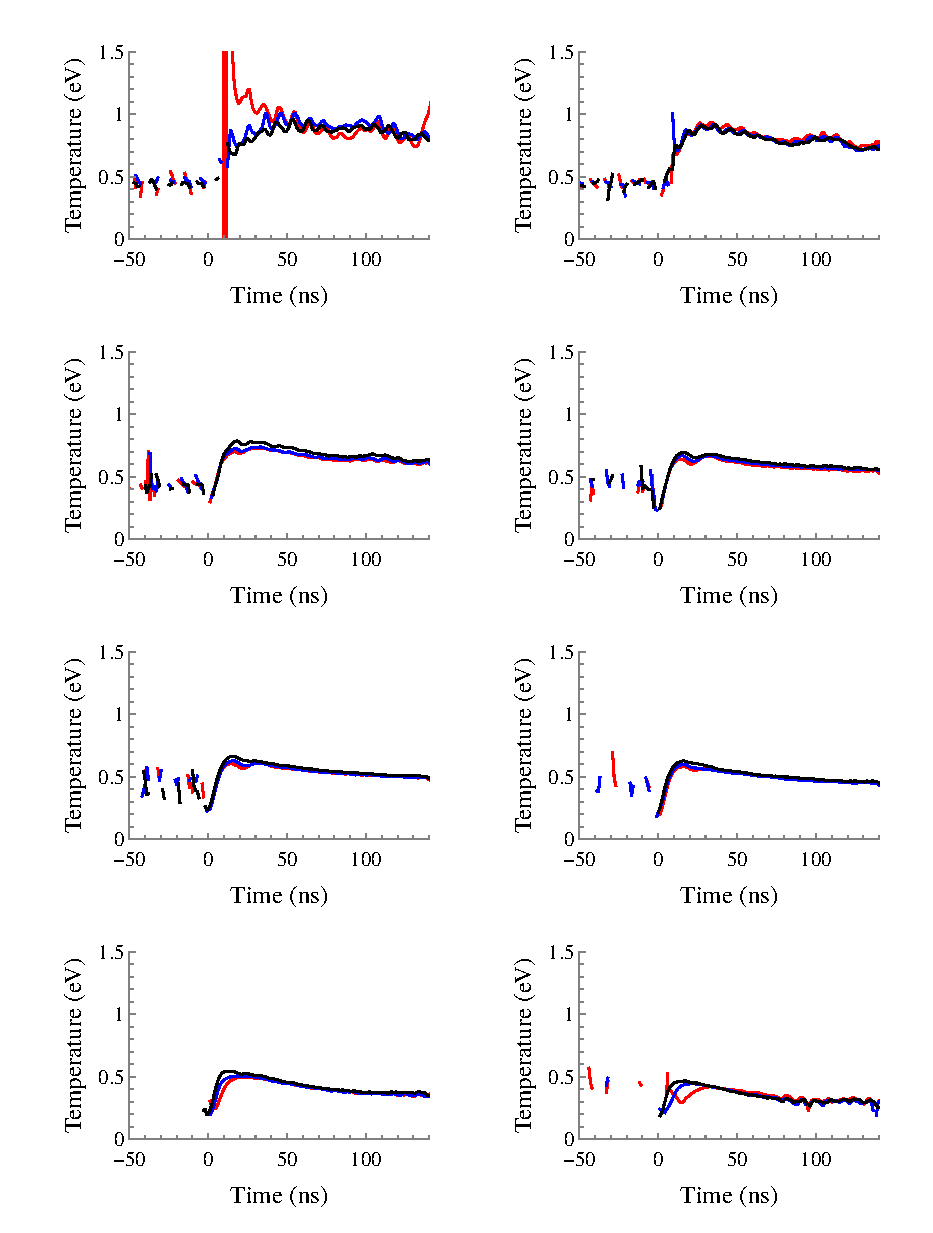
\includegraphics{./chapters/emissions/figures/boltplots.eps}
  \caption{These aren't as good as I had hoped$\ldots$}
  \label{fig:boltplots}
\end{figure}


\section{Global Model Comparison}



\section{Summary}
